\documentclass{article}

\usepackage[T2A]{fontenc}
\usepackage[utf8]{inputenc}
\usepackage[russian]{babel}
\usepackage{commath}
\usepackage{amsmath}
\usepackage{amsfonts}
\usepackage{mathtools}
\usepackage{amssymb} 
\usepackage{parskip}
\usepackage{titling}
\usepackage{color}
\usepackage{hyperref}
\usepackage{cancel}
\usepackage{enumerate}
\usepackage{graphicx}
\usepackage[a4paper, left=2.5cm, right=1.5cm, top=2.5cm, bottom=2.5cm]{geometry}

\graphicspath{ {./images/} }
\setlength{\droptitle}{-3cm}
\hypersetup{
    colorlinks=true, %set true if you want colored links
    linktoc=all,     %set to all if you want both sections and subsections linked
    linkcolor=blue,  %choose some color if you want links to stand out
}

\pagenumbering{arabic}

\begin{document}
    \section{Действительные числа}
        \subsection{Введение. Задача измерения отрезков}
            $a_{\in \mathbb{N}} + x = b_{\in \mathbb{N}}$ есть алгебраическая предпосылка для возникновения целых чисел.
            
            $\mathbb{Z} = N^{+} \cup N^{-} \cup \{0\}$
            
            Свойства для $\mathbb{N}$ сохраняем в $\mathbb{Z}$:

            \begin{enumerate}
                \item $a + b = b + a$
                \item $a + (b + c) = (a + b) + c$
                \item $ab = ba$
                \item $a(bc) = (ab)c$
                \item $a(b + c) = ab + ac$
            \end{enumerate}
            
            $a_{\in \mathbb{Z} \textrm{\textbackslash} \{0\}}x = b_{\in \mathbb{Z}}$ есть алгебраическая предпосылка для возникновения рациональных чисел $Q$
            
            O------------------------A\\
            O-----E
            
            $OE$ --- единичный отрезок

            $\abs{OA} = n \abs{OE}$
            
            \textbf{Определение.} Отрезки $a$ и $b$ называются соизмеримыми, если $\exists$ отрезок $c$:
            
            $\abs{a}=n\abs{c}$\\
            $\abs{b}=m\abs{c}$, $m,\ n \in \mathbb{N}$

            $\abs{a} = \frac{n}{m}\abs{b}$
            
            \textbf{Определение.} Числа вида $\frac{n}{m}$, где $m \in \mathbb{N},\ n \in \mathbb{Z}$ назовем рациональными.

            \underline{Между любыми двумя рациональными числами $\exists\ \infty$ число других рациональных чисел}

            Например, между $r_1$ и $r_2$ существует $\frac{r_1 + r_2}{2}$ и т.д.

            \underline{Множество $\mathbb{Q}$ --- ``всюду плотно``} 

            \underline{Существуют несоизмеримые отрезки:}

            Нарисуем квадрат со сторонами $x$ и $y$.
            $x^2$ + $x^2$ = $y^2$.
            Если они соизмеримы, то $y = rx$.
            $\not\exists\ r \in \mathbb{Q}: r^2 = 2$

            От противного:

            Пусть $\exists\ r = \frac{n}{m}$ --- несократимая $\Rightarrow \frac{n^2}{m^2} = 2 \Rightarrow n^2 = 2m^2 \Rightarrow n = 2k \Rightarrow 4k^2 = 2m^2 \Rightarrow 2k^2 = m^2 \Rightarrow m^2 \vdots 2 \Rightarrow m \vdots 2 \Rightarrow$ дробь сократима --- противоречие.

            \underline{Это возникновение иррациональных чисел}

        \subsection{Бесконечные десятичные дроби}
            Будем рассматривать десятичные дроби:
            \begin{enumerate}
                \item конечная десятичная дробь.\\
                $\abs{OA} = 4,806 = 4_{= 4\ \abs{OE}_{= e}} + \frac{8}{10} + \frac{6}{1000}$\\
                \item $\abs{OA} = \frac{1}{3}?$\\
                $\frac{1}{3} = \frac{m}{10^n} \quad 10^n = 3m$ невозможно\\
                Но можно измерять со все больше возрастающей точностью\\
                $|_{0}----|----|_{N}----|_{N+1}---->$\\
                $O-----------A$\\
                \begin{enumerate}[1.]
                    \item Делим $OX$ на отрезки равные 1, т.е. рассмотрим $[n; n+1] \Rightarrow$ пусть $A$ попала в $[N; N+1]$
                    \item $|_{N}--|--|_{A}--|--|_{N}--|_{N+1}$\\
                    $[N,m_1;N,m_1 + \frac{1}{10}]$\\
                    $[N,n_1;N,n_1 + \frac{1}{10}]$ --- это тот куда попал $A$\\
                    $[N,n_1n_2;N,n_1n_2 + \frac{1}{100}]$ и т.д.\\
                \end{enumerate}
            \end{enumerate}

        $[N; N+1] = I_0$\\
        $[N,n_1; N,n_1 + \frac{1}{10}] = I_1$\\
        $[N,n_1n_2; N,n_1n_2 + \frac{1}{100}] = I_2$\\
        $...$\\
        $[N,n_1n_2...n_k; N,n_1n_2...n_k + \frac{1}{10^k}] = I_k$\\
        $...$\\
        Это процесс(*)!!!

        $I_0 \supset I_1 \supset I_2 \supset ... \supset I_k \supset ...$

        $\alpha_k = N,n_1n_2...n_k \quad \nearrow$

        $\alpha_k' = N,n_1n_2...n_k + \frac{1}{10^k} \quad \searrow$ 

        \textbf{Определение.} Этот процесс (*) принято называть бесконечной десятичной дробью и обозначается\\ 
        $\alpha N,n_1n_2...n_k...$
        
        \textbf{Определение.} Число $\alpha_k = N,n_1n_2...n_k$ --- приближение $\alpha$ по недостатку с точностю до $\frac{1}{10^k}$

        \textbf{Определение.} Число $\alpha_k' = N,n_1n_2...n_k + \frac{1}{10^k}$ --- приближение $\alpha$ по избытку с точностю до $\frac{1}{10^k}$

        В общем случае процесс (*), кроме случая конечной десятичной дроби.

        Например:
        \[0,45\]
        \[[0,4; 0,5]\]
        \[\textrm{процесс раздвоился}\]
        \[[0,44; 0,45]\quad|\quad[0,45; 0,46]\]
        \[[0,449; 0,450]\quad|\quad[0,450; 0,451]\]
        \[[0,4499; 0,4500]\quad|\quad[0,4500; 0,4501]\]
        \[...\]
        \[\cancel{0,44999...(9)} \textrm{(такие числа не рассматриваем)}\quad\quad 0,4500000...(0)\]

        \textbf{Определение.} Положительным действительным числом называем всякую бесконечную десятичную\\ дробь, не оканчивающуюся последовательностью 9-ок.

        \textbf{Определение.} Число $\beta$ назовем отрицательным действительным числом, если $\beta = -\alpha = -N,n_1n_2...n_k...$

        $0 = 0,000...0...$\\
        $\cancel{0 = -0,000...0...}$

        $\alpha = [\alpha_k; \alpha_k']$

        $-\alpha = \beta = [-\alpha_k'; -\alpha_k]$

        \textbf{Свойства.}

        \begin{enumerate}[0.]
            \item Действительные числа можно сравнивать
            \begin{enumerate}[1.]
                \item \[\alpha, \beta > 0;\ \alpha = N,n_1n_2...n_k...;\ \beta = N,m_1m_2...m_k...\]
                \[N < M \Rightarrow \alpha < \beta, N = M, N > M \Rightarrow \alpha > \beta\]
                \[\Downarrow\]
                \[n_1 < m_1 \Rightarrow \alpha < \beta, n_1 = m_1, n_1 > m_1 \Rightarrow \alpha > \beta\]
                \[\Downarrow\]
                \[...\]
                \item \[\alpha < 0, \beta > 0 \Rightarrow \alpha < \beta\]
                \item \[\alpha < 0, \beta < 0 \Rightarrow \alpha > \beta \Leftrightarrow -\alpha < -\beta\]
            \end{enumerate}
        \end{enumerate}

        \subsection{Рациональные числа и бесконечные десятичные дроби}
        \textbf{Утверждение.} Всякое рациональное число можно записать в виде бесконечной десятичной дроби. 

        $\frac{2}{5} = 0,4(0)...$

        $\frac{5}{11} = 0,(45)...$

        $\frac{1}{7} = 0,(142857)...$

        $\frac{8}{45} = 0,1(7)...$

        \textbf{Определение.} Период - повторяющаяся группа цифр.

        \textbf{Определение.} Длина периода - число цифр.

        \textbf{Утверждение.} Всякое рациональное число представимо в виде \underline{периодической} бесконечной десятичной дроби.

        $\uparrow$ Достаточно доказать для правильных дробей.

        $\frac{m}{n}$

        Остатки при делении на $n$?

        $0_{\textrm{с этим легко}}, 1, 2, 3, 4, ..., n - 1$

        Остался $n - 1$ остаток

        Не более чем через $n - 1$ чисел возникает второй раз остаток, который уже был. Далее остатки будут повторяться.

        \underline{Итог:} Иррациональные числа - непериодические бесконечные десятичные дроби. 

        \subsection{Разделяющее число числовых множеств}
        Некоторую совокупность действительных чисел назовем числовым множеством.
        
        Само множество действительных чисел обозначается $\mathbb{R}$.
        
        Другими примерами числовых множеств могут служить:
        
        $\mathbb{R}+$ —-- множество положительных действительных чисел.
        
        $\mathbb{Q}-$ —-- множество отрицательных рациональных чисел.
        
        $(-\infty; a]$ —-- множество действительных чисел $x: x \leq a$.

        \textbf{Определение.} Числовое множество $X$ называется ограниченным, если $\exists\ M \in \mathbb{R}: \forall\ x \in X: \abs{x} \leq M$.

        \textbf{Определение.} Будем говорить, что множество $B$ лежит справа от множества $A$, если $\forall\ x \in A$ и $\forall\ y \in B: x \leq y \quad A, B \subset \mathbb{R}$.

        % КОНЕЦ ЛЕКЦИИ №18

        \textbf{Определение.} Число $c \in \mathbb{R}$ называется разделяющим числом для множества $A$ и $B \subset \mathbb{R}$, если $\forall\ a \in A$ и $\forall\ b \in B: a \leq c \leq b$.

        Из определения следует, что если для множеств $A$ и $B$ существует разделяющее число, то $B$ лежит справа от множества $A$. Верно и обратное утверждение.

        \textbf{Теорема.} Пусть $A$ и $B$ два числовых множества. Причем множество $B$ лежит справа от множества $B$.\\
        Тогда $\exists$ по крайней мере одно число $c$, разделяющее эти множества.

        $\uparrow$
        Рассмотрим единичные отрезки вида $[n,n+1]$.
            
        Для множества $B$ рассмотрим самый левый из отрезков $[n,n+1]$, содержащий элементы этого множества (если самый маленький $b$ попал на границу, то берем «достаточный отрезок»). Обозначим этот отрезок $[N,N+1]$. Для простоты будем считать, что $N \geq 0$.
        
        Для множества $A$ рассмотрим самый правый из отрезков $[n,n+1]$. Пусть это $[M,M+1]$. 

        \begin{enumerate}
            \item $M > N$ --— невозможно (так как тогда есть $a > b$);
            \item $M < N$ —-- тогда в качестве разделяющего числа можно взять, например, $c = N. \forall\ a \in A, \forall\ b \in B a \leq c \leq b$.
            \item $M = N \Rightarrow$ 
        \end{enumerate}

        Разделим $[N,N+1]$ на $10$ частей $\Rightarrow [N + \frac{n_1}{10},N + \frac{n_1 + 1}{10}], n_1 = 0,1,2,...,9$.

        Снова выбираем $N_1: [N + \frac{N_1}{10},N + \frac{N_1 + 1}{10}]$ —-- самый левый (с замечанием) из таких отрезков, содержащий элементы из $B$, и $M_1: [N + \frac{M_1}{10},N + \frac{M_1 + 1}{10}]$ --— самый правый из таких отрезков, содержащий элементы из $A$. 

        \begin{enumerate}
            \item $M_1 > N_1$ --— невозможно (так как тогда есть $a > b$);
            \item $M_1 < N_1$ —-- тогда в качестве разделяющего числа можно взять, например, $c = N,N_1. \forall\ a \in A, \forall\ b \in B a \leq c \leq b$.
            \item $M_1 = N_1 \Rightarrow$ 
        \end{enumerate}

        Полученный $[N + \frac{N_1}{10},N + \frac{N_1 + 1}{10}] = [N,N_1; N,N1+1/10]$ снова делим на $10$ частей. И снова выбираем самый левый промежуток, содержащий элементы из $B$, и самый правый, содержащий элементы из $A$. И т.д.

        В итоге, мы либо найдем $c$, либо в самом «тяжелом случае» построим систему вложенных промежутков: 

        $[N,N + 1] \supset [N,N_1; N,N_1 + \frac{1}{10}] \supset [N,N_1N_2; N,N_1N_2 + \frac{1}{100}] \supset ...$

        Возьмем в качестве $c$ б.д.д., отвечающую этому процессу: $c = N,N_1N_2...N_k...$

        Это $c$ и будет разделяющим числом.
        
        Действительно, покажем, что $\forall\ b \in B c \leq b$.

        От противного. Если существует $b < c$, то из упорядоченности действительных чисел при большом $l$ точки $b$ и $c$ попали бы в разные отрезки длины $\frac{1}{10^l}$, и выбранный малый промежуток не был бы самым левым для множества $B. \Rightarrow c \leq b$

        Аналогично $\forall\ a \in A a \leq c$.

        Остались неосвещенными моменты: $c$ оканчивается последовательностью 9-ок, для $N < 0$. $\downarrow$

        \subsection{Теорема о разноцветных отрезках (единственность разделяющего числа)}
        \textbf{Определение.} Пусть множество $B$ лежит справа от $A$. Назовем отрезок $[a; b]$ разноцветным, если $a \in A, b \in B$.

        \textbf{Определение.} Будем говорить, что существует система сколь угодно малых разноцветных отрезков, если $\forall\ \varepsilon > 0$ (каким бы маленьким мы его не взяли) $\exists$ разноцветные отрезки $[a; b]$ и $[\alpha; \beta]$ ($[\alpha; \beta] \supset [a; b], \alpha, \beta$ --— рациональные числа): $\beta - \alpha < \varepsilon$. 

        \textbf{Замечание.}

        \begin{enumerate}
            \item Так как $\forall\ \varepsilon$, то таких отрезков сколь угодно много (система).
            \item Координаты $\alpha, \beta$ —-- рациональные числа нужны нам, так как действия с действительными числами ещё не вводились. Мы не знаем, что есть $a - b$. Если бы знали, то просто писали бы: $\exists$ разноцветные отрезки $[a; b]: b - a < \varepsilon$.
        \end{enumerate}

        \textbf{Теорема.} Пусть множество $B$ лежит справа от $A$. Для того, чтобы $A$ и $B$ разделялись лишь одним числом необходимо и достаточно, чтобы $\exists$ система сколь угодно малых разноцветных отрезков. 

        $\uparrow$ Необходимость ``$\Leftarrow$``. Пусть существует система сколь угодно малых разноцветных отрезков, покажем, что $\exists! c$. 

        От противного. Пусть $\exists$ два разделяющих числа $c_1$ и $c_2$ (для определенности $c_1 < c_2$). При достаточно большом $n$ числа $c_1$ и $c_2$ принадлежат отрезкам деления числовой оси длины $\frac{1}{10^n}$, не имеющими общих концов (это следует из упорядоченности действительных чисел). Т.е. между $c_1$ и $c_2$ существует хотя бы один отрезок $[\frac{m}{10^n}; \frac{m + 1}{10^n}]: c_1 < \frac{m}{10^n} < \frac{m + 1}{10^n} < c_2$.
        
        Но тогда, $\forall\ a \in A, b \in B a \leq c_1 < c_2 \leq b$, а потому $d = $(длина любого отрезка с рациональными концами, содержащего $[a; b]$) $> \frac{1}{10^n}$. Противоречие с существованием системы сколь угодно малых разноцветных отрезков.

        Достаточность ``$\Rightarrow$``. Пусть $\exists! c$, покажем существование системы сколь угодно малых разноцветных отрезков.

        $c$ --— единственное разделяющее число. Зададим $\varepsilon > 0$ и возьмём $[\alpha, \beta]$ c рациональными концами такой, что $\alpha < c < \beta$. Например, если $c_n$ --— приближение $c$ по недостатку с точностью до $\frac{1}{10^n}$, то можем рассмотреть целую систему таких промежутков: $[\alpha_n; \beta_n] = [c_n - \frac{1}{10^n}; c_n + \frac{1}{10^n}]$. 

        Покажем, что на любом отрезке такого вида есть, хотя бы одно число из $A$. От противного: пусть нет, тогда $\forall\ a \in A a < \alpha_n$, при этом $\forall\ b \in B b \geq c$. Тогда все числа из $[\alpha_n; c]$ разделяют $A$ и $B$. Аналогично, можно показать, что на любом отрезке такого вида есть, хотя бы одно число из $B$. Значит любой такой $[\alpha_n; \beta_n] \supset [a_n; b_n]$ --- разноцветный.

        $\beta - \alpha = \frac{2}{10^n} < \{10^n = (1 + 9)^n > 9n\} < \frac{2}{9n} < \varepsilon_k < \varepsilon$, где $N \geq [\frac{2}{9 \varepsilon_k}] + 1. \downarrow$ 

        \textbf{Пример.} Покажем, что отрезки $[1; 4] [4; 8]$ разделяются лишь числом $4$.
        
        Заметим, что отрезки $[4 - \frac{1}{n}; 4 + \frac{1}{n}]$ —-- разноцветные. Их длина $d = \frac{2}{n}$ путем выбора $n$ может быть сделана меньше любого наперед заданного действительного $\varepsilon$. Если $\frac{2}{n} < \varepsilon_k < \varepsilon$, то $n \geq [\frac{2}{\varepsilon_k}] + 1$. 

        \textbf{Пример.} Найти разделяющее число множеств $A = \{ \frac{n^2}{n^2 + 1}, n \in \mathbb{N} \}$ и $B = \{ \frac{n^2 + 2}{n^2 + 1}, n \in \mathbb{N} \}$

        Заметим, что $\frac{n^2}{n^2 + 1} = \frac{n^2 + 1 - 1}{n^2 + 1} = 1 - \frac{1}{n^2 + 1} < 1, \frac{n^2 + 2}{n^2 + 1} = \frac{n^2 + 1 + 1}{n^2 + 1} = 1 + \frac{1}{n^2 + 1} > 1$. Т.е. множество $B$ лежит справа от $A$. Докажем, что $1$ --- единственное разделяющее число этих множеств. Отрезки $[1 - \frac{1}{n^2 + 1}; 1 + \frac{1}{n^2 + 1}]$ разноцветные, их длина $d = \frac{2}{n^2 + 1} < \frac{2}{n^2} < \frac{1}{n} < \varepsilon_k < \varepsilon \Rightarrow n \geq [\frac{2}{\varepsilon_k}] + 1$.

        \subsection{Арифметические операции над действительными числами}

        \textbf{\underline{Сложение}}
        
        Пусть заданы $x, y \in \mathbb{R}$. Рассмотрим два множества:

        $A = \{p + q, \textrm{ где } p \in \mathbb{Q}, p \leq x, q \in \mathbb{Q}, q \leq y\}$, 

        $B = \{r + s, \textrm{ где } r \in \mathbb{Q}, r \geq x, s \in \mathbb{Q}, s \geq y\}$.

        Так как $p \leq x \leq r$, $q \leq y \leq s \Rightarrow p + q \leq r + s$, значит множество $B$ лежит справа от $A \Rightarrow$ существует по крайней мере одно разделяющее число для этих множеств. 

        \textbf{Утверждение.} Покажем, что разделяющее число существует единственное.

        Для этого достаточно показать существование системы сколь угодно малых разноцветных отрезков. 

        Пусть десятичное приближение по недостатку с точностью $\frac{1}{10^n}$ для $x$ --— это $\frac{l}{10^n}$, а для $y$ --— $\frac{m}{10^n}$. Тогда $\frac{l}{10^n} \leq x < \frac{l + 1}{10^n}$, $\frac{m}{10^n} \leq x < \frac{m + 1}{10^n}$. Тогда $\frac{l}{10^n} + \frac{m}{10^n} \in A$, а $\frac{l + 1}{10^n} + \frac{m + 1}{10^n} \in B$. Но $d = (\frac{l + 1}{10^n} + \frac{m + 1}{10^n}) - (\frac{l}{10^n} + \frac{m}{10^n}) = \frac{2}{10^n} < \frac{2}{9n} < \varepsilon_k < \varepsilon$. Т.е. существуют сколь угодно маленькие разноцветные отрезки. 

        Это единственное число, разделяющее множества $A$ и $B$, называют суммой $x + y$.

        \textbf{Определение.} Суммой действительных чисел $x$ и $y$ называют такое число $x + y$, которое является единственным разделяющим числом для сумм $p + q (p \leq x, q \leq y, p,q \in \mathbb{Q})$ и сумм $r+s (r \geq x, s \geq y, r,s \in \mathbb{Q})$.
        
        \textbf{\underline{Разность}}

        \textbf{Определение.} Разностью действительных чисел $x$ и $y$ назовем сумму $x$ и $(-y)$.
        
        \textbf{\underline{Умножение}}

        (I)

        $x, y > 0$

        $A = \{pq, p, q \in \mathbb{Q}^{+}: p \leq x; q \leq y\} (*)$

        $B = \{rs, r, s \in \mathbb{Q}^{+}: x \leq r; y \leq s\} (*)$

        Легко понять, что $pq \leq rs \Rightarrow B$ лежит справа от $A \Rightarrow \exists$ хотя бы одно разделяющее число $c$.

        \textbf{Утверждение.} $\exists! c$ для $A$ и $B$ (*)

        (II)

        Если $x, y$ не $> 0$, то произведение вводится в соответствии с правилом знаков. 

        $(-x)y = x(-y) = -xy$

        и 

        $(-x)(-y) = xy$

        Свойства (доказываются из свойств рациональных чисел):

        \begin{enumerate}
            \item $xy = yx$
            \item $x(yz) = (xy)z$
            \item $x(y + z) = xy + xz$
        \end{enumerate}

        Остается в силе:

        $0 * x = x * 0 = 0, \forall\ x \in \mathbb{R}$

        $1 * x = x * 1 = x, \forall\ x \in \mathbb{R}$

        \textbf{\underline{Деление}}

        $x > 0$ Поймем, что есть $\frac{1}{x}$

        $A = \{\frac{1}{p}, p \in \mathbb{Q}^{+}: p \geq x\}$ (**)

        $B = \{\frac{1}{q}, q \in \mathbb{Q}^{+}: q \leq x\}$ (**)

        $q \leq p \in \mathbb{Q}^{+} \Rightarrow \frac{1}{p} \leq \frac{1}{q} \Rightarrow$ множество $B$ лежит справа от $A$.
        
        $\Downarrow$

        $\exists$ хотя бы одно разделюящее число.

        \textbf{Утверждение.} $\exists! c$ для $A$ и $B$ (**)

        Если $x = 0: \not\exists\ \frac{1}{x}$
        
        Если $x < 0: \frac{1}{x} = -\frac{1}{-x}$

        $x, y \in \mathbb{R}:\quad y \neq 0 \quad \frac{x}{y} = x*(\frac{1}{y})$

        Свойство:

        $x*\frac{1}{x} = 1 \quad \forall x \neq 0$

        Множество $\mathbb{R}$ замкнуто относительно четырех арифметических операций.

        $\mathbb{R}$ --- числовое поле.

        \subsection{Превращение бесконечных периодических десятичных дробей в обыкновенные}

        \textbf{Пример.}
        
        $0,(54)$

        $x = 0,(54)$

        $100x = 54,(54)$

        $99x = 54$

        $x = \frac{54}{99} = \frac{6}{11}$

        \textbf{Пример.}

        $0,(351)$

        $x = 0,(351)$

        $1000x = 351,(351)$

        $999x = 351$

        $x = \frac{351}{999}$

        \textbf{Пример.}

        $0,47(612)$

        $x = 0,47(612)$

        $x * 10^5 = 47612,(612)$

        $x * 10^2 = 47,(612)$

        $x = \frac{47612 - 47}{10^2 * 999}$

        \subsection{Рациональное и иррациональное число. Плотность этих множеств в R}
        \textbf{Утверждение.} Для $\forall\ x, y \in \mathbb{R} \exists$ отрезок с рациональными концами: он лежит между $x$ и $y$. (***)

        $\uparrow$

        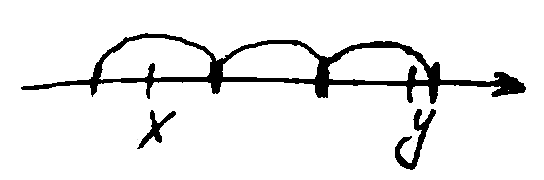
\includegraphics[scale=0.2]{d_ch_8}

        $x, y \in \mathbb{R}, x < y$

        $\exists$ разбиение отрезками длины $\frac{1}{10^n}$, что $x$ и $y$ лежат в отрезках такой длины и не имещих общих концов: это отрезки вида $[\frac{m}{10^n}_{ = r \in \mathbb{Q}}; \frac{m + 1}{10^n}] = [r, r + \frac{1}{10^n}] \downarrow$
        
        \textbf{Утверждение.} Между любыми $x, y \in \mathbb{R}, x \subset y \exists\ \infty$ число рациональных чисел.

        $\uparrow$

        Уже в утверждении (***) показали, что $\exists$ между $x$ и $y$ $[r_{\in \mathbb{Q}}, r + \frac{1}{10^n}_{\in \mathbb{Q}}] = [r_1, r_2] \Rightarrow r_1 < \frac{r_1 + r_2 = r_3}{2} < r_2$

        $r_1 < \frac{r_1 + r_3}{2} < r_3 < \frac{r_3 + r_2}{2} < r_2$ и т.д. $\downarrow$

        \textbf{Утверждение.} Между $x$ и $y \in \mathbb{R} x < y \exists\ \infty$ число иррациональных чисел.

        $\uparrow$

        Покажем, что между любыми двумя рациональными числами $\exists$ хотя бы одно иррациональное.

        Уже между $x$ и $y \exists\ [r, r + \frac{1}{10^m}] = [r_1, r_2]$ 

        $r_1 = \alpha,\alpha_1\alpha_2...\alpha_m \quad r_2 = r_1 + \frac{1}{10^m}$

        Легко понять, что $\beta = \alpha,\alpha_1...\alpha_m00100111$ (допишем заведомо непериодический конец) $\downarrow$

        \textbf{Определение.} Числовое множество $A$ эквивалентно множеству $B$, если $\exists$ взаимнооднозначное отображение $A$ в $B$.

        \textbf{Определение.} Числовое множество $A$ называется счетным, если оно эквивалентно множеству $\mathbb{N}$. (т.е. все элементы $A$ можно пронумеровать).

        \textbf{Утверждение.} Множество рациональных чисел счётно. 

        $\uparrow$

        \underline{Способ 1} $\frac{p}{q}$ --- рациональное, если $p \in \mathbb{Z}, q \in \mathbb{N}$

        $s = \abs{p} + q$ --- высота рационального числа.

        $s = 1 \quad \frac{0}{1} \quad 1 $ист

        $s = 2 \quad \frac{1}{1} - \frac{1}{1} \cancel{\frac{0}{2}} \quad 3$ ист

        $s = 3 \quad \frac{\pm 2}{1} \frac{\pm 1}{2} \cancel{\frac{0}{3}} 5$ ист

        $s:$ не более $2(s - 1) + 1 = 2s - 1$ ист --- конечное число и т.д. все занумерую.

        \underline{Способ 2} 
        --- - линия, вдоль которой нумерую, вычеркивая повторяющиеся.

        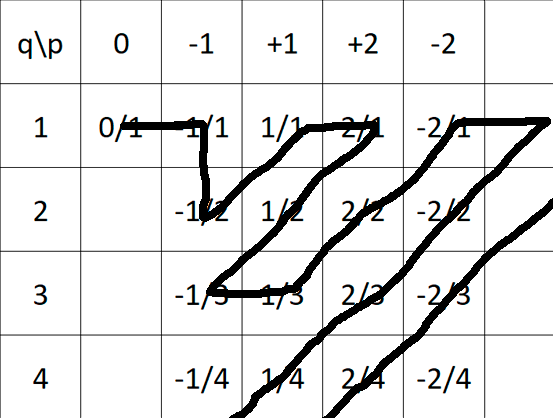
\includegraphics[scale=0.4]{d_ch_8_1}

        $\downarrow$

        \textbf{Утверждение.} Множество $\mathbb{R}$ --- несчетное множество.

        $\uparrow$

        Остается пологать, что (0; 1) --- несчетное множество.

        От противного. Пусть счетное, тогда нумерую все элементы.

        Обозначим эту группу (****)

        $r_1 = 0,a_{11}a_{12}a_{13}...a_{1n}...$

        $r_2 = 0,a_{21}a_{22}a_{23}...a_{2n}...$

        $r_3 = 0,a_{31}a_{32}a_{33}...a_{3n}...$

        $r_n = 0,a_{n1}a_{n2}a_{n3}...a_{nn}...$

        и т.д.

        $\beta = 0,\beta_1\beta_2...\beta_n...$

        $\beta_1 \neq a_{11} \neq 9 \Rightarrow \beta \neq r_1$
        
        $\beta_2 \neq a_{22} \neq 9 \Rightarrow \beta \neq r_2$
        
        $\beta_3 \neq a_{33} \neq 9 \Rightarrow \beta \neq r_3$

        и т.д.

        $\beta \neq r_n, n \in \mathbb{N}$

        т.е. $\beta \not\in (****)$ --- противоречие со счетностью (0, 1) $\downarrow$

        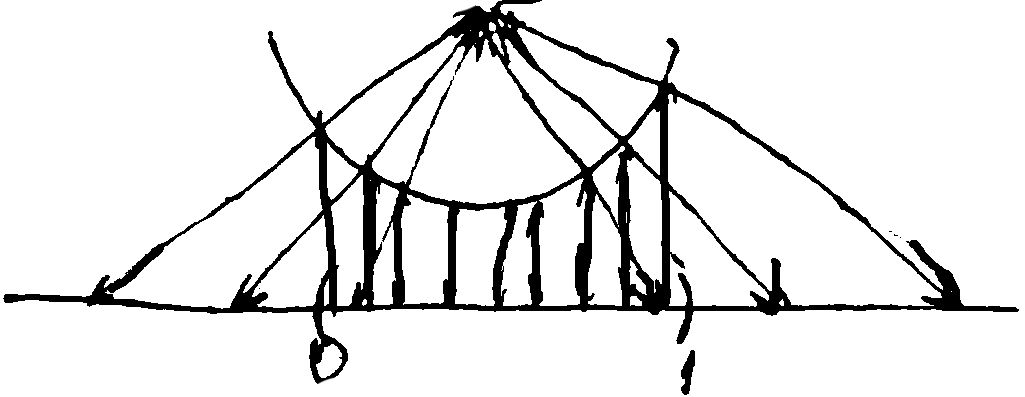
\includegraphics[scale=0.15]{d_ch_8_2}

        $(0, 1)$ эквивалентно $\mathbb{R}$

        $\mathbb{R}_{\textrm{несчет.}} = \mathbb{Q}_{\textrm{счет.}} \cup \overline{\mathbb{Q}} \Rightarrow \overline{\mathbb{Q}}$ несчетная.

\end{document}